% ==========================================================================
%	RESEARCH PROPOSAL
% ==========================================================================

% - INTRODUCTION -----------------------------------------------------------
\chapter{Introduction}
\label{ch:intro}
% --------------------------------------------------------------------------

	\section{Motivation} \label{sec:intro-motivation}
	
	\ac{cc} has become a critical method of consuming \ac{it} infrastructure, for private users and enterprises across the globe: Per Arcserve, around 100 zettabytes of data will be stored in the cloud by 2025, which will account for approx. 50\% of all data in the world. \cite{Morgan2020} Furthermore, Gartner predicts that the worldwide public cloud service end-user spending will amount approx. \$482 billion US dollars by the end of 2022, increased by approx. 65\% over the course of just two years \cite{Rimol2021}. Additionally, around 90\% of large enterprises have adopted a multi-cloud infrastructure. This results in 53\% of \ac{it} decision-makers saying that this strategy helps them achieve their business goals \cite{Forrester2022}. In conclusion, from business, economic, and technical standpoints, the importance of \ac{cc} has been and still is on the rise.
	
	However, crucial downsides and challenges can not be overseen when considering the adaptation of cloud infrastructure within businesses: Less than half of traditional small businesses use cloud infrastructure or hosting services \cite{DigitalOcean2021}, with security, compliance, and data protection issues representing the leading challenges and concerns. \cite{ISC22022}\cite{Flexera2021}
	
% --------------------------------------------------------------------------	
	
	\section{Problem Statements} \label{sec:intro-problems}
	
	With different service and deployment models, \ac{cc} vendors have recognized these issues and implement features and aids that claim to reduce or fully mitigate these challenges. On the other hand, commercial \ac{cc} dates back almost 20 years \cite{Qian2009}, as the mentioned challenges and concerns do. Looking at the slow adaptation of \ac{cc} in traditional businesses and the continuously present fear of security issues, the trust in the security mechanisms seems not be built yet. 
	\\\ \\\
	This proposed Master's thesis recognizes the following subset of problems:
	
	\paragraph{P1}\label{p1} There exist several information security challenges that apply to the domain of \ac{cc}, some of which are unique to the \ac{cc} architecture.
	
	\paragraph{P2}\label{p2} Reducing or mitigating these security challenges imposes a significant complexity and resource overhead.
	
	\paragraph{P3}\label{p3} Private cloud architecture is, by mistake, generally considered more secure than public cloud architecture.
	\\\ \\\
	These problems will be addressed in this thesis' contributions, outlined in the following.

% --------------------------------------------------------------------------

	\section{Contribution} \label{sec:intro-contribution}
	
	The following list of contributions aims at addressing or solving the problems stated previously in \autoref{sec:intro-problems}.
	
	\paragraph{C1}\label{c1} (i) Discover and describe current, relevant information security challenges that apply to \ac{cc}, (ii) link them to affected \ac{cc} deployment and service models, (iii) as well as to their corresponding mitigation, reduction, or defense mechanisms.
	
	\paragraph{C2}\label{c2} Perform case studies on security defense mechanisms given by exemplarily chosen \ac{cc} offerings that address the corresponding information security challenges from \nameref{c1}.
	
	\paragraph{C3}\label{c3} Evaluate the case studies from \nameref{c2} in terms of security defense functionality existence, operation, limitation, as well as introduction of new challenges.
	
	\paragraph{C4}\label{c4} For challenges that apply to both private and public cloud offerings, additionally compare the findings and evaluation of their security functionality.
	\\\ \\\
	The aspired contributions can be directly linked to the problems:
	
	\nameref{p1} will be addressed by a comprehensive analysis of current information security challenges and its classification to \ac{cc} service and deployment models, given by \nameref{c1}.
	
	By performing distinct case studies across different \ac{cc} offerings (cf. \nameref{c2}) and evaluating their outcomes (cf. \nameref{c3}), \nameref{p2} will be addressed.
	
	Finally, by comparison of case study results that apply to public and private cloud infrastructure (combination of \nameref{c3} and \nameref{c4}), \nameref{p3} will be addressed.
	
	Additionally, it can be seen that the contributions are built on top of each other, resulting in individual contributions that receive added value when considered in total.
	
% --------------------------------------------------------------------------

	\section{Proposal Structure} \label{sec:intro_structure}
	
	This section outlines the structure of the remaining research proposal document. \\\
	
	\autoref{ch:foundations} presents the necessary foundational information required to discuss and understand the proposed research in terms of \ac{cc} and information security terminology definitions, properties and characteristics.
	
	\autoref{ch:related-work} discusses the research that is already in place with regards to the topic at hand, deducts limitations of that research and describes how these limitations are addressed by the contribution of this thesis.
	
	\autoref{ch:approach} defines the methodology of the contribution development for its three phases (discovery, testing implementation, and evaluation) as well preliminary assumptions, limitations and risks to this research.
	
	Finally, \autoref{ch:organization} outlines the research stakeholders, Master's thesis artefacts as well as the project plan of this work.
		
%	In order to contribute to this topic, a set of research questions is defined, built on top of one another. Proceeding with a top-down approach, the first question is what current security, compliance, and data protection challenges are within the discipline of \ac{cc}.
%	
%	The answers will form the foundation for the second question regarding the applicability of the challenges to the various service and deployment models of \ac{cc}. Based on this classification, the actual research contribution to the topic at hand can be performed.
%	
%	The challenges and, more importantly, the reduction or mitigation measures will be practically examined based on an evaluation framework that will be designed and exemplarily applied on chosen \ac{cc} solutions. Specifically, the following questions will be asked:
%	
%	\begin{itemize}
%		\item Does a mitigation or reduction functionality exist with the given \ac{cc} solution within its scope?
%		\item If it exists, does it sufficiently tackle the challenge?
%		\item If it exists, does it create new challenges in the given \ac{cc} solution within or outside its scope?
%		\item What can be done to enhance mitigation or reduction of a given issue (even further)?
%	\end{itemize}
%	
%	The findings on various challenges from the disciplines of security, compliance, and data protection, applied on the different \ac{cc} service and deployment models, will then conclude the final question, being if the overall rationale of safety concerns with regard to \ac{cc} is justified.
%	
%	It is expected that the findings from the research to be performed will open up new questions and possibilities for follow-up research.

% - FOUNDATIONS ------------------------------------------------------------
\chapter{Foundations}
\label{ch:foundations}
% --------------------------------------------------------------------------

This chapter gives an overview on the necessary background information and technical foundations required to perform the described research. It is expected that these foundations will be elaborated in the actual thesis more thoroughly as certain examined aspects of the research might require additional background.

% --------------------------------------------------------------------------

	\section{Introduction to \Acl{cc}} \label{sec:foundations-intro_cc}
		The U.S. \ac{nist} defines \ac{cc} as ``a model for enabling ubiquitous, convenient, on-demand network access to a shared pool of configurable computing resources (...) that can be rapidly provisioned and released with minimal management effort (...).`` \cite{NISTcc} It can be seen as the latest form of infrastructure consolidation after the introduction of client-server computing and the rise of datacenter hardware virtualization. \cite[p.\ 1]{Kumar2018}
		
		In general, \ac{cc} is described by a vendor-consumer relationship, with the vendor being the provider of the \ac{it} resources, and the consumer being the receiver and user of those resources. Depending on the deployment model of the \ac{cc} infrastructure at hand, the vendor can be 
		
		\begin{itemize}
			\item internal to an organization or providing isolated resources exclusively to that organization (i.e., \textit{private cloud}),
			\item external, providing resources to multiple entities (i.e., \textit{public cloud}),
			\item or a mix of both (cf.\ \autoref{subsec:foundations-intro_cc-deployment}). \cite{NISTcc}
		\end{itemize}  
		
		The service level defines the level of abstraction of the resources to the consumer and which party is responsible for which layer of application provisioning and deployment (cf.\ \autoref{subsec:foundations-intro_cc-service}). \cite{NISTcc}
		
		The \ac{nist} laid out several aspects that further define \ac{cc} characteristics, service, and deployment models.
		
		
		\subsection{Characteristics} \label{subsec:foundations-intro_cc-characteristics}
			\begin{description}
				\item[On-demand self-service] Provisioning of (more) computing, storage, network resources, etc. is done by the consumer without interaction with the \ac{cc} service provider. \cite{NISTcc} This implies a form of automation on the \ac{cc} vendor's end as well as the existence of control and monitoring interfaces for the consumer. \cite[p.\ 51]{Kumar2018} 
				\item[Broad network access] The \ac{cc} vendor's services and capabilities are accessible over the network and can be accessed via mechanisms that are already in place for consuming clients. \cite{NISTcc}\cite[p.\ 45]{Kumar2018}
				\item[Resource pooling] Resource pooling allows \ac{cc} vendor's to introduce the concept of \textit{multi-tenancy}, where the physical infrastructure that is made available is virtualized and dynamically assigned to distinct consumers, or \textit{tenants}, based on demand or contractual agreements. \cite{NISTcc}\cite[p.\ 45]{Kumar2018} In other words, a \textit{pool} of total resources present is made available to multiple consumers based on their \textit{current} needs and re-evaluated over the course of the usage.
				\item[Rapid elasticity] The consumer can dynamically scale their resource capacity up or down as needed. The consumer is not aware of any global resource limitations which make the \ac{cc} resources appear unlimited. \cite{NISTcc}
				\item[Measured service] The consumed services are quantitatively measured by the \ac{cc} vendor for billing, controlling and optimization purposes. This is based on appropriate forms of metering with regard to the service (e.g., number of terabytes of storage consumed within a month). Thus, billing of utilized services is often done on a pay-per-use basis. \cite{NISTcc} Consequently, the more resources are utilized by the vendor, the higher the cost. This process is transparent to both vendor and consumer, allowing for consumption and billing monitoring, control, and reporting. \cite{NISTcc}
			\end{description}
			
		
		\subsection{Deployment Models} \label{subsec:foundations-intro_cc-deployment}
		The deployment model of \ac{cc} defines by whom the infrastructure can be consumed.
		
		\begin{description}
			\item[Public Cloud] The infrastructure provisioned is subject to public use and is owned and managed by a cloud service provider or \ac{cc} vendor, residing in their location. \cite{NISTcc} Here, depending on contractual agreements, multi-tenancy across individual entities can take place. Notable vendors include \textit{\ac{aws}}, \textit{Microsoft Azure}, as well as \textit{\ac{gcp}}.
			\item[Private Cloud] The infrastructure provisioned is subject to exclusive use by one entity or organization. Hence, no multi-tenancy is taking place between multiple entities. The physical infrastructure can reside within the premises of the organization, be located in a consolidated data center or managed by a third party exclusively to the consumer. \cite{NISTcc} There exist exclusive private cloud deployments, as well as offerings by public cloud vendors that aim to bring their experience to the private cloud (e.g., \ac{aws} \textit{Virtual Private Cloud (VPC)}).
			\item[Hybrid Cloud] The consumer utilizes two or more distinct \ac{cc} infrastructures (private or public) that remain self-sufficient individually but can be consolidated to achieve the consumer's infrastructural needs. \cite{NISTcc} An organization can design their hybrid cloud environment individually or make use of commercial offerings, e.g. \textit{\acs{hpe} GreenLake}.
		\end{description}
		
		Apart from these three deployment definitions, \ac{nist} also mentions the \textit{community cloud} model that is shared by a community of consumers with shared concerns and requirements. \cite{NISTcc}  Additionally, \textit{multi-cloud} environments describe the usage of multiple public or private cloud infrastructures for different purposes, reasons, or advantages, depending on their use cases within the organization. These two deployment models will play a subordinary role in this proposed work.

		
		\subsection{Service Models} \label{subsec:foundations-intro_cc-service}
			The service models of \ac{cc} lay out the \ac{it} resources' level of abstraction to the consumer and define the provisioning and deployment responsibilities between the vendor and the consumer. This is exemplarily presented in \autoref{fig:foundations-cc-service-models} below by means of the deployment of an arbitrary application. 
		
		\begin{figure}[h!]
			\centering
			\includegraphics[width=\linewidth]{content/2-research-proposal/img/RedHat_2020_IaaS PaaS SaaS Diagram.png}
			\caption{\acl{cc} service model comparison \cite{RedHatServiceimg}}
			\label{fig:foundations-cc-service-models}
		\end{figure}
	
		The blue-colored disciplines are subject to the consumer whereas the red-colored disciplines are to be done by the vendor. Each subsequent service model contains the vendor responsibilities of the previous model.  Note that the lefthand side of the Figure also includes a comparison to a traditional on-premises infrastructure where the consumer is responsible for the entire provisioning and deployment. 
		
		\begin{description}
			\item[\acf{iaas}] The virtualized \ac{it} infrastructure is provided by the vendor. The consumer is responsible for the provisioning of the resources by means of operating system, runtime, up to the application itself. Management of the hardware infrastructure cannot be performed by the consumer. \cite{NISTcc} The consumer receives generic infrastructure, e.g., a \ac{vm}, that needs to be fully set up for its intended purposes.
			\item[\acf{paas}] Apart from all \ac{iaas} aspects being provided by the vendor, the \ac{paas} infrastructure is already provisioned by means of the adequate operating system, application runtime and services that allow for the specific deployment of applications appropriate to that platform. \cite{NISTcc} For instance, the vendor might receive \ac{paas} infrastructure to deploy a Java application without the need of preparing the infrastructure for supporting Java. The consumer cannot change or manage the underlying environment, but only use it to deploy their application and perform limited platform configuration. \cite{NISTcc}
			\item[\acf{saas}] Apart from the underlying infrastructure that is required to run an application, \ac{saas} also delivers the actual software to be used by the consumer. \cite{NISTcc} Consequently, the vendor is in charge of administering all layers of the stack, including \ac{it} infrastructure, its provisioning, and software deployment. The consumer has access to the software instance (e.g., via a thin client) as well as limited configuration capability, but cannot change the software deployment itself. \cite{NISTcc}
		\end{description}
		
		Apart from these \ac{nist} definitions, there have been movements to go beyond the scope of \ac{saas}, referring to a paradigm called \textit{\ac{xaas}}. This term itself has not been yet well-defined as it is being used by different entities to describe different events in the evolvement of \ac{cc}. \cite{Duan2015}\cite{Robison2008} However, it can be generalized that \ac{xaas} refers to all \ac{it} activities and services that are being or will be migrated into the \ac{cc} paradigm based on latest \ac{it} achievements that do not fit the aforementioned service model descriptions \cite{Duan2015} (e.g., \textit{Artificial Intelligence as a Service}, \textit{High Performance Computing as a Service}, etc.). Furthermore, it could also include service-oriented disciplines that go beyond consumption of \ac{it} resources. \cite{Doerner2011}
		
% --------------------------------------------------------------------------
				
	\section{Information Security} \label{sec:foundations_it-security}
		
	The \ac{nist} defines information security as ``the protection of information and information systems from unauthorized access, use, disclosure, disruption, modification, or destruction in order to ensure confidentiality, integrity, and availability.`` \cite{Nieles2017} The last three characteristics can be further defined:
		
	\begin{description}
		\item[Confidentiality] Unauthorized entities are restricted from access and disclosure of information for the purpose of protecting personal privacy and proprietary information. \cite{Nieles2017}  
		\item[Integrity] Improper modification or destruction of information, including the compromitation of data non-repudiation and authenticity, is protected against. Furthermore, \textit{data integrity} means that data has not been improperly altered, whereas \textit{system integrity} goes beyond unautorized manipulation, defining system function quality when performing as intended and unimpaired. \cite{Nieles2017} 
		\item[Availability] Accessibility and usability of information is reliable and timely. \cite{Nieles2017} This also includes the prevention of intended, unauthorized withholding of data. \cite[p. 36]{FischerHuebner2001}
	\end{description}
		
	This \textit{CIA triad} can be extended by additional characteristics, e.g. \textit{accountability} (user actions can be traced back to them), \textit{functionality} (system's behavior is as intended and expected) and \textit{reliability} (system always performs under equal conditions). \cite[p. 36 sq.]{FischerHuebner2001}
		
	The terms \textit{information security}, \textit{cyber security}, \textit{\ac{it} security}, etc., are often used interchangeably in literature. Nevertheless, each of these disciplines is based on the aforementioned \textit{CIA triad}.
		
	Furthermore, additional terms need to be introduced to understand information security.
		
	\begin{description}
		\item[Vulnerability] A weakness within a system that could be exploited by a threat source. \cite{Nieles2017}
		\item[Threat] An event or circumstance that could exploit a system's vulnerability to be carried out. \cite{Nieles2017}
		\item[Risk] A measure of impact of a potential threat and its likelihood to occur. \cite{Nieles2017}
	\end{description}
		

% - RELATED WORK -----------------------------------------------------------
\chapter{Related Work} 
\label{ch:related-work}
% --------------------------------------------------------------------------
As mentioned in the \nameref{ch:intro}, the discipline of security in the domain of \ac{cc} has been and remains highly important for organizations and research. Consequently, there has been a substantial amount of scientific work already put into the security examination that is briefly outlined in the following. \\\

\section{Present Research} \label{sec:related-work_present}

As \ac{cc} leverages a vast amount of distinct \ac{it} services, Hashizume et al. \cite{Hashizume2013} discovered that they also inherit these services' distinct security flaws. This is especially true for \textit{niche} solutions outside of traditional infrastructure and platform offerings that go beyond web applications, data hosting, or virtualization. They also underline that different service models (cf. \autoref{subsec:foundations-intro_cc-service}) present themselves with distinct security flaws. They also point out that the biggest concerns lie in infrastructure services (i.e., storage, virtualization, and networks). Multi-tenancy is also named as a primary risk as it allows multiple users (that potentially do not know each other, let alone their individual intentions) to share the same physical hardware.

The previous aspect of multi-tenancy issues is also portrayed by Khalil et al. \cite{Khalil2014}. Based on their research, they were able to find 28 distinct threats and vulnerabilities, categorized in five critical domains, namely security standards, network, access, cloud infrastructure, and data. They have also examined the potential of targeted attacks, such as denial of service, phishing, etc. However, they do not distinguish vulnerabilities that come from human error (such as infrastructure misconfiguration) on the consumer's end, and fundamental vulnerabilities subject to the vendor's responsibility. In terms of threat mitigation, they found out that current security standards could reduce the risk of security breaches but create a substantial computing overhead, leading to higher operational cost.

Loske \cite[p. 25]{Loske2015} was able to conduct an analysis of currently perceived cloud risks and link them to the CIA traid as well as to additional risk dimensions (i.e., performance, accountability, and maintainability). 

Qian et al. \cite{Qian2009} additionally point out that utilizing a public cloud requires taking risk into account that lies outside of the responsibilities of the consuming organization, including internet connectivity issues, cloud vendor power outages, service disruptions, etc. This is mitigated by cloud vendors implementing service level agreements, but cannot be fully ruled out in practice.

This process of trust rebalancing when utilizing public \ac{cc} is also mentioned by A. Singh et al. \cite{Singh2017}. Their research also identifies multi-tenancy and other novel features unique to \ac{cc} as the top vulnerability source.

Apart from the aforementioned third-party dependency that is imposed when choosing public \ac{cc}, Y. Zhang et al. \cite{Zhang2012} mention the fact that public cloud vendors are also more receptive to cyber attacks as it is known that they store a vast amount of data that could be leveraged for malicious activities. Similar to the previous works, their findings again focus on issues introduced by multi-tenancy.

Research conducted by Paxton \cite{Paxton2016} ties in with the previous findings of multi-tenancy issues and is extended by analyzing the potential of data breaches and highjacking of accounts. Here, adequate counter-measures are identified (segmentation, \ac{vm} introspection, data loss prevention tools, proper identity access management), but lie in the implementation responsibility of the consumer. Cited studies show that only the minority of consumers implement these countermeasures.

Focussing on private cloud infrastructure, Manakattu et al. \cite{Manakattu2020} discovered that implementing private \ac{cc} can benefit security by residing inside an exclusively internal network. However, this is only the case if the internal network is already well-secured and constantly improved and audited. Again, the introduction of \ac{cc} concepts (e.g., multi-tenancy) could also be exploited in the private network and thus need to be additionally addressed by the security framework of the implementing organization.

Following the statement that private cloud infrastructure can be generally seen as more secure, Felsch et al. \cite{Felsch2015}  analyzed multiple open-source private cloud distributions on the security of their control interfaces. They found that several distributions could be compromised through that interface, one of them even granting unauthorized root access to \acp{vm}. This was possible by making the control interfaces accessible from the Internet.

There have been efforts to develop unified solutions that address security, compliance and/or data protection challenges in the cloud, e.g., by Song et al. \cite{Song2012}. Their approach is to offer data protection \textit{as a service} that could be implemented by cloud vendors and be consumed side-by-side to the actual cloud service. They recognize that different domains and use cases require different architectures. However, the development of such and other mechanisms and their implementation by cloud vendors could move security-related responsibilities away from the consumer who might benefit from it, especially if security expertise is not fully available to them. \\\

\section{Achievements \& Limitations} \label{sec:related-work_limitations}

Based on the findings of the evaluation of the related work to that topic, it can be seen that a lot of effort has been put into discussing and partially solving information security issues within the domain of \ac{cc}. Most importantly, the authors were able to point out and prioritize different security challenges. Specifically, the majority of research done  states that new concepts introduced \textit{because of} \ac{cc} impose a top-priority security risk in the domain of \ac{cc}, with multi-tenancy and extensive virtualization being mentioned most frequently. 

Furthermore, some authors also evaluate their findings practically by applying them on the specific domain of \ac{cc}. There have also been developments of distinct solutions that are supposed to address their previously inconclusively addressed problems. 

However, several gaps in the examined research can be seen. First of all, with the emergence of cloud services that go beyond traditional provisioning of resources, new information security challenges could occur. This is mentioned in the presented research, but not thoroughly examined. Moving on, several statements point out that security implementation remains a requirement on the consumer's end or, at least, makes the consumption of \ac{cc} less convenient by imposing a high complexity and resource overhead. Again, the presented research does not perform case studies examining the existence and behaviour of exemplarily chosen cloud offerings across different service and deployment models. Moreover, a comparison between supposedly similar features across multiple cloud offerings might also be interesting. Finally, the over-simplified assumption of public cloud offerings being blanket \textit{less secure} than private cloud infrastructure is known and addressed, but not within a practical manner by means of comparison.

In summary, the following research limitations are identified:

\paragraph{L1}\label{l1} Most recent emergence of \ac{cc} might have yielded new information security challenges that are not currently addressed.
\paragraph{L2}\label{l2} Current research does not perform test implementation analyses on existing security features regarding existence, operationality, and limitation \textit{across different \ac{cc} offerings, service and deployment models}.
\paragraph{L3}\label{l3} Following from \nameref{l2}, there are no current \textit{comparisons} between security features across their applicable \ac{cc} offerings and deployment models.
\paragraph{L4}\label{l4} Because of the lack of comparison, the \textit{security dilemma} between \ac{cc} deployment models (i.e., private and public clouds) is known but not examined yet.
\\\ \\\
The proposed Master's thesis' research aims at addressing and potentially solving these research gaps, outlined in the following.

\section{Application of Contribution} \label{sec:related-work_contribution}

The research gaps presented in \autoref{sec:related-work_limitations} can be  applied to the deduced problems from \autoref{sec:intro-problems}. Specifically, most relevant and recent cloud security challenges (cf. \nameref{l1}) define a subproblem of the overall existence of perceived cloud security issues (cf. \nameref{p1}). The problem of cloud security complexity and resource overhead, given by \nameref{p2} might be solved by addressing \nameref{l2} and \nameref{l3} by means of practical test implementation and evaluation. The security misconception across deployment models (cf. \nameref{p3}) is also not examined yet, as stated in \nameref{l4}.

As the individual contributions of this proposed research are deducted from the problems, they can also be transitively applied on the gaps, resulting in the following relationships.

\begin{itemize}
	\item \textbf{\nameref{p1}} might benefit from addressing \textbf{\nameref{l1}} which will be achieved by \textbf{\nameref{c1}}.
	\item \textbf{\nameref{p2}} might benefit from addressing \textbf{(\nameref{l2} and \nameref{l3})} which will be achieved by \textbf{(\nameref{c2} and \nameref{c3})}.
	\item \textbf{\nameref{p3}} might benefit from addressing the results from \textbf{(\nameref{l2} and \nameref{l3}), combined with \nameref{l4}}, which will be achieved by the results of \textbf{(\nameref{c2} and \nameref{c3}), combined with \nameref{c4}}.
\end{itemize}

% - APPROACH ---------------------------------------------------------------
\chapter{Approach} 
\label{ch:approach}
% --------------------------------------------------------------------------

	\section{Research Structure \& Methodology} \label{sec:approach-structure}
	This section will describe the necessary steps to achieve the described contributions of this research, presented in \autoref{sec:intro-contribution}. This will be achieved by performing three consecutive phases, namely the \textit{discovery}, the \textit{testing implementation}, and the \textit{evaluation}, outlined and reasoned in the following.
	
	\subsection{Discovery Approach} \label{sec:approach-structure-discovery}
	
	In {\autoref{ch:related-work}, it has been shown that a substantial amount of research is dedicated to security challenges in the domain of \ac{cc}. The proposed Master's thesis will tie in with that research, performing a more extensive literature analysis to describe and summarize risks within \ac{cc}. Following \nameref{c1}, the focus will lie on recent and relevant cloud security issues. However, for the sake of coherence, as well as to achieve the subsequent contributions, it will also include well-known, but not exemplarily and comparatively evaluated risks. This step will finally produce a descriptive list of relevant security issues within the \ac{cc} domain, as required by \nameref{c1} (i). 	
	
	Following that one-dimensional list of risks, these will then be classified by means of their applicability to the service and deployment models of \ac{cc}. This might, again, be aided by literature review, or be performed based on justified deductions on the applicability of the risk. This will result in mappings of risks-to-service model and risks-to-deployment model, and potentially a conjoined mapping of all three dimensions, addressing \nameref{c1} (ii). 
	
	These mappings will be then used for a last discovery step that will examine theoretical security defense functions that are required to address the individual security issues, resulting in a service and deployment model-aware issue-to-defense function mapping, e.g.
	
	\begin{center}
		``Security Issue A \textit{applies to} \ac{iaas} deployments in the Public Cloud and \textit{could be mitigated by} Defense Mechanism A.``\\
	\end{center}
	
	These mappings will satisfy \nameref{c1} (iii).
	
	It is expected that the findings will require a refinement of the \nameref{ch:foundations} and \nameref{ch:related-work} chapters, which is also included in the discovery phase. 
		
	It can be expected that the discovery findings will become more extensive than bearable for the scope of a Master's thesis, which is why the focus will lie on perceived risks that can be practically evaluated with the means of the evaluation framework (cf. \autoref{subsec:approach-structure-evaluation}) and this work's predefined limitations (cf. \autoref{sec:approach-assumptions}).
	
	Another possible form of discovery methodology would be performing targeted surveys. However, this is linked to a number of challenges. First, this research aims at covering a significant amount of problem statements. That is, trying to understand \ac{cc} security challenges for different offerings, service and deployment models as well as allowing for comparability of these findings. Additionally, it is expected that test subjects are not aware of all currently relevant security challenges in the domain of \ac{cc}, resulting in biases and distortion from the start. In order to allow for comparability and reduce bias, an unbearable amount of test subjects would be needed. This is why an objective literature analysis, as stated above, is preferred.

	
	\subsection{Testing Implementation Approach} \label{subsec:approach-structure-testing}
	
		\subsubsection{Case Study Design Framework}
		
		The output from the discovery phase, satisfying \nameref{c1}, will be used as input for the testing implementation, which aims at satisfying \nameref{c2}. Specifically, the findings of cloud security issues, mapped to their applicable service and deployment model as well as to their defense mechanism(s) need to be put under test in terms of exemplarily chosen \ac{cc} deployments. This will be done by designing individual case studies that practically examine the functionality of the defense mechanisms. These will predefine an implementation environment and goal with regards to the security aspect. The implementation will include, but is not necessarily limited to
		
		\begin{itemize}
			\item deployment of resources that can consume the defense mechanism,
			\item configuration of the mechanism,
			\item testing of its intended functionality within its scope,
			\item testing of functionality impairment of the deployment,
			\item and so on.
		\end{itemize}
		
		All findings within the process will be documented for the purpose of the evaluation phase. In case a defense mechanism applies to multiple service or deployment models, the case study will be performed for each model individually. In any case, a defense mechanism will be evaluated for every exemplarily chosen cloud offering, if available. This will yield results satisfying \nameref{c2} and serve as input for \nameref{c3} and \nameref{c4}.
		
		As the concrete mechanisms under test will be defined during the actual research, a fine-grade case study design cannot be presented yet. This means that the bullet points above might be limited or extended, depending on the individual case.
		
		Furthermore, it can be expected that the limitations and risks of this research (cf. Sections \ref{sec:approach-assumptions} and \ref{sec:approach-risk}) might limit the practical performance of the case studies, i.e., the testing environment does not provide all means to perform the desired case study in a practical manner. To mitigate this issue, the case study will be performed on a theoretical basis by making use of literature, documentation, etc. that will attest the functionality of the affected defense mechanism. Nevertheless, this inconvenience might result in distortion which needs to be taken into account during the evaluation phase.
		
		Again, another reasonable form of testing methodology would be performing usability tests. As this research covers an expert-level topic (i.e., configuration and application of information security mechanisms in the domain of \ac{cc}), this would require the presence of a significant number of expert users. Considering the different \ac{cc} offerings under test, the test subjects would require, at least, basic knowledge of the testing environments, which cannot be expected, let alone guaranteed. Failure to find an appropriate number of expert test users might, again, lead to biases and distortions that could render the evaluation less conclusive. It is also necessary to mention that usability testing could only cover a part of \nameref{c2}, namely the usability aspect of perceived complexity. In any case, limitations and further challenges might need additional methodology outside of usability testing to be properly addressed. This is why the case study development and testing implementation will be comprehensively done by the author.
			
		\subsubsection{\acs{cc} Offerings under Test} \label{subsubsec:approach-structure-testing-offerings}
	
		The following \ac{cc} offerings will be used exemplarily for the application of the case study design framework. The choice is justified by the accessibility of the platforms. Additionally, these platforms are chosen based on their representability for their deployment model. \acs{hpe} GreenLake is chosen based on the corporate environment of this research. 
		
			\paragraph{Public Cloud: \textit{\acf{aws}}} \ac{aws} has got the highest market share in terms of public cloud infrastructure and services.\footnote{as per \textit{Synergy Reserach Group}: \url{https://www.srgresearch.com/articles/as-quarterly-cloud-spending-jumps-to-over-50b-microsoft-looms-larger-in-amazons-rear-mirror}} It offers a tier of its services free of charge.\footnote{\url{https://aws.amazon.com/free/}}
			\paragraph{Private Cloud: \textit{OpenStack} by the Open Infrastructure Foundation}  OpenStack's ecosystem is strongly growing as many enterprises state that they are currently or about to implement OpenStack\footnote{as per various cited institutions: \url{https://www.openstack.org/analysts/}}. OpenStack allows for a light-weight private cloud deployment in terms of a developer sandbox environment\footnote{\url{https://docs.openstack.org/devstack/latest/}}.
			\paragraph{Hybrid Cloud: \textit{\acs{hpe} GreenLake} by \acl{hpe}} \acs{hpe} GreenLake is the in-house solution of the sponsoring company of this proposed Master's thesis. \ac{hpe} provides near production-grade deployments that will mainly be used for the testing implementation.\footnote{\url{https://www.hpe.com/us/en/greenlake.html}} However, if limitations occur for specific case studies, the corresponding business unit is expected to provide further resources for their practical implementation. \\\
	
		It should be noted that, based on its definition (cf. \autoref{subsec:foundations-intro_cc-deployment}), a hybrid cloud contains aspects of both public and private clouds. Therefore, the majority of the evaluation will presumably be done on the private aspect of the offering. At the time of the creation of this proposal, it is unclear which components of the \ac{hpe} GreenLake offering will be put under evaluation.
	
	\subsection{Evaluation Approach} \label{subsec:approach-structure-evaluation}
	
		\subsubsection{Individual Evaluation} \label{subsubsec:approach-structure-evaluation-individual}
		
		The findings from the testing implementation phase will now be evaluated individually in order to satisfy \nameref{c3}. This will be done by means of a \textit{Goal-Question-Metric} (GQM) plan with the following criteria:
		
		\paragraph{Goal [G1]: \textbf{Evaluate existence of security defense mechanism}\label{g1}}
			\begin{description}
				\item[Question] Does a security defense mechanism exist for its corresponding security challenge 	within the scope of the presented case study?
				\item[Metric] Possibility of implementation [yes/no] \\
			\end{description}
		
		
		\paragraph{Goal [G2]: \textbf{Evaluate possibility and extent of security defense mechanism configuration}\label{g2}}
		
		\begin{description}
			\item[Question] Can the security defense mechanism be configured by the user? If so, to which extent does the user have power over the configuration?
			\item[Metric] Possibility of configuration [yes/no], extensiveness of configuration [amount of settings, quantified by impact] \\
		\end{description}
		
		
		\paragraph{Goal [G3]: \textbf{Evaluate configuration responsibility}\label{g3}}
		
		\begin{description}
			\item[Question] Which security configuration aspects are subject to the user's responsibility, which aspects are covered by the provider?
			\item[Metric] Documented configuration steps of provider's responsibility, put in quantified ratio to configuration step's available to the user \\
		\end{description}
		
		
		\paragraph{Goal [G4]: \textbf{Evaluate configuration complexity}\label{g4}}
		
		\begin{description}
			\item[Question] How complex is the security mechanism complexity presumed by an idealized user? 
			\item[Metric] Difference from default configuration [number of configuration steps], type of configuration interface [UI/CLI/API], documentation of security mechanism configuration [descriptive] \\
		\end{description}
		
		
		\paragraph{Goal [G5]: \textbf{Evaluate security mechanism's resource overhead}\label{g5}}
		
		\begin{description}
			\item[Question] Does a resource overhead exist if the security mechanism is applied, as opposed to if it is not applied? 
			\item[Metric] Applicable resource and performance metrics put in relation [additional resource consumed, additional cost] \\
		\end{description}
		
		
		\paragraph{Goal [G6]: \textbf{Evaluate security mechanism's limitations}\label{g6}}
		
		\begin{description}
			\item[Question] Does the security defense mechanism present itself with limitations within its scope of operation?
			\item[Metric] comparison between intended and actual operation [descriptive] \\
		\end{description}
		
		
		\paragraph{Goal [G7]: \textbf{Evaluate the introduction of new challenges if security mechanism is used}\label{g7}}
		
		\begin{description}
			\item[Question] Does the security defense mechanism lead to the introduction of new challenges within or outside its scope of operation?
			\item[Metric] comparison between intended and actual operation [descriptive] \\
		\end{description}
		
		The evaluation goals are partly built on top of each other. Specifically, the subsequent evaluation after \hyperref[g1]{G1} is only possible if \hyperref[g1]{G1} itself yields a positive answer. \hyperref[g3]{G3} and \hyperref[g4]{G4} are also only reached if \hyperref[g2]{G2} is evaluated positively.
		
		The findings of the mentioned evaluation criteria will be summarized and used for the formulation of recommendations for action, an outlook, as well as future research to \ac{cc} security. All in all, these goals within the individual evaluation of case studies aim at satisfying \nameref{c3}.	
		
		\subsubsection{Comparative Evaluation} \label{subsubsec:approach-structure-evaluation-comparative}
		
		For all case studies that can be performed on multiple deployment environments, an additional comparative evaluation is performed. This evaluation takes the individual findings into account, as described in \autoref{subsubsec:approach-structure-evaluation-individual}. The qualitative and quantitative differences between the individual deployments will be established and assessed. Specifically, the comparison of \hyperref[g4]{G4} between public and private cloud deployments will benefit the achievement of \nameref{c4}. However, the comparison of all metrics will aid the contribution. These findings will be added to the formulation of recommendations for action, outlook, and future research possibilities in the domain of \ac{cc} security. \\\
		
		It is expected that performing the actual case studies, as described in \autoref{subsec:approach-structure-testing}, will yield additional interesting questions in terms of individual and comparative assessment, which is why the aforementioned GQM plan definition might be extended during the actual research.
	
%	The evaluation of the risk-to-service model and risk-to-deployment mappings is visualized in \autoref{fig:approach-eval_process-framework} on the next page and explained further in the page after.
%	
%	\newpage
%	\vfill
%	\begin{figure}
%		\centering
%		\includegraphics[width=0.75\linewidth]{content/2-research-proposal/img/eval-framework.pdf}
%		\caption{Preliminary Evaluation Framework Outline}
%		\label{fig:approach-eval_process-framework}
%	\end{figure}
%	\vfill
%	\clearpage
%	
%	The document or note icons correspond to deliverables that are required by the cascading research questions stated in \autoref{sec:intro-contribution}. The process starts with the input of the previously mentioned findings to the applicable cloud service or deployment models. 
%	
%	After that, the first evaluation question is answered, whether a counter-measure to the described risk is in place, depicted in blue color. 
%	
%	If so, the process moves to the mitigation or reduction analysis, depicted in green color. Here, an intermediate step is introduced that allows for a complexity evaluation of the corresponding risk. That is, whether the complexity of the risk is within scope and boundaries of the Master's thesis in terms of its practical evaluation, further described in \autoref{sec:approach-assumptions}. If so, the evaluation is performed on a practical level with an individually designed, short functional case study, depicted as a black box in the Figure. If not, the evaluation is performed on theoretical grounds by examining the intended functionality of the counter-measure based on documentation, literature, etc. Either way, this analysis aims at answering the second evaluation question, whether and how well the mechanism actually mitigates or reduces the risk.
%	
%	The third question, depicted in orange color, whether limitations or new challenges occur due to the counter-mechanism, is, again, answered by deduction. Potentially, specific use cases also allow for a practical evaluation of that question. 
%	
%	Finally, the fourth and last evaluation question deals with the potential of further improvement, depicted in purple color. If the first question was answered negatively, the process automatically moves to the last question, as it can be expected that the non-existence of counter-measures might be improved to mitigate or reduce it. Conversely, it is expected (and \textit{hoped for}), that this path does not need to be taken.
%	
%	The answers of questions one through four will then finally serve as inputs for an overall conclusion of current justified security, compliance, and data protection risks. \\\

% --------------------------------------------------------------------------

	\section{Assumptions and Limitations} \label{sec:approach-assumptions}
	
	As certain limitations might not be clear until the start of the actual Master's thesis development, this list of assumptions and limitations makes no claim to be exhaustive.
	
	\begin{description}
		\item[Lack of Budget] At the time of creating this research proposal, it is expected that the research to-be-conducted will not receive any financial support which might be beneficial to the evaluation of paid services or offerings.
		\item[Closed Scope] The practical evaluation will take place on the pre-selected cloud platforms as mentioned in \autoref{subsubsec:approach-structure-testing-offerings}. Deviations of functionality and provided mechanisms from other offerings can therefore not be considered for the final evaluation.
		\item[Environmental Limitations] The practical evaluation can only be applied to the \textit{available} cloud platform environments. For instance, if a public cloud risk can only be evaluated in terms of an \ac{aws} paid service, the risk cannot be considered for further evaluation.
		\item[Operational Correctness \& Integrity] As this research does not aim at revealing operational issues of the exemplarily chosen \ac{cc} offerings, it is expected that the deployments perform as intended by the provider. Especially, it is assumed that public and hybrid cloud vendors that offer their services within an environment outside of the presenting testing framework's influence, function as documented and implement all security standards. 
		\item[Attack Simulation] Consequently, evaluation of risks that require actual attack simulation cannot be carried out either as non-local environments will impose boundaries to these attacks that remain far beyond the scope of this work. Plus, practical cyber attack expertise cannot be expected from the author of this proposed research.
		\item[Little \ac{saas} Consideration] It can be expected that \ac{saas} offerings will not be provided by any of the chosen evaluation platforms (for \ac{aws}, presumably at least not free of charge), which is why the aforementioned evaluation framework will be mainly applied onto \ac{iaas} and \ac{paas} offerings.
	\end{description}
	
	Overall, further limitations to the scope and complexity of this proposed research are expected as for the given nature of Master's thesis, that is, a limited working time frame of six months, a generally limited amount of content pages (approx. 60-80 pages), and the fact that the work is conducted in a cooperative study manner next to a full-time employment as given by the study program of the HECTOR School.

% --------------------------------------------------------------------------

	\section{Risk to the Research and Mitigation} \label{sec:approach-risk}
	
	As certain risks to this proposed work might not be clear until the start of the actual Master's thesis development, this list of risks and risk mitigations makes no claim to be exhaustive. It does also not contain superior risks outside of the scope of the research and outside the control of the stakeholders (e.g., sickness, emergency situations, etc.). 
	
	\begin{description}
		\item[Misrepresentation of Research Novelty] The analysis of the related work (cf. \autoref{ch:related-work}) has been and will be done to the best of the author's knowledge and belief, especially in terms   of describing the present research's limitations. However, it is possible that relevant work is disregarded (e.g., due to unavailability, etc.) that might render this research's contributions less novel than they were expected.
		\item[Environment Exhaustion] There is a possibility that the available lightweight or free-tier environments of the \ac{cc} offerings will not provide all necessary functionality required to perform a practical evaluation in terms of the evaluation framework (cf. \autoref{sec:approach-eval_process}). This could be mitigated by deviating to a theoretical evaluation. Specifically for the evaluation of \ac{hpe} GreenLake, there might be the possibility of a more advanced deployment for this research's purposes. As the specific evaluation input is not given yet, it is also unclear whether the test environment will suffice.
		\item[Out-of-Scope Practical Complexity for Relevant Risks] Thus less likely, there is a possibility that a significant number of relevant risk analyses, that should preferably be carried out practically, will demonstrate with increased evaluation complexity. It is desired to have both theoretical and practical evaluations, but depending on the complexity and relevance of given risks, there might be trade-offs in the practical evaluation for the sake of demonstration.
	
	\end{description}

% - ORGANIZATION -----------------------------------------------------------
\chapter{Planning}
\label{ch:organization}
% --------------------------------------------------------------------------
	
	\section{Research Stakeholders} \label{sec:organization-stakeholders}
	
	The Master's thesis will be conducted by \textbf{Oliver Rudzinski} (oliver.rudzinski@hpe.com).
	\begin{description}
		\item[KIT affiliation] M.Sc. Candidate for Information Systems Engineering and Management at the HECTOR School of Engineering and Management (Technology Business School of the KIT)
		\item[\ac{hpe} affiliation] Infrastructure Technology Architect for the \textit{Value Solutions} department at the \acl{hpe} Sales Center GmbH in Berlin, Germany. 
	\end{description}
	
	The following stakeholders affiliated with the Karlsruhe Institute of Technology are identified.
		
	\begin{description}
		\item[Reviewer] Prof. Dr. Ralf Reussner (ralf.reussner@kit.edu)
		\item[Second Reviewer] Dr. Robert Heinrich (robert.heinrich@kit.edu)
	\end{description}
	
	Additionally, as the Master's thesis will be conducted in cooperation with the author's employer, the following stakeholder(s) affiliated with \ac{hpe} are identified.
	
	\begin{description}
		\item[Manager] Markus Leitzgen | Inside Sales Manager \textit{Value Solutions} (markus.leitzgen@hpe.com) 
	\end{description}
	
	It shall be noted that additional subject-matter experts, closely related to the \ac{hpe} GreenLake business unit, might be brought in for supporting purposes, or out of interest to their business.	

% --------------------------------------------------------------------------

	\section{Artefacts} \label{sec:organization-deliverables}
	This section outlines the artefacts that are expected to be developed during the process of the Master's thesis:
	
	\begin{itemize}
		\item Research Proposal (this document)
		\item Master's thesis Colloquium presentation slides
		\item Master's thesis
	\end{itemize}
	
	In case any source code or configuration files are created during the evaluation process of this research, they will be included in adequate manner.
	
	Furthermore, it is expected that the findings of this research will also be presented to an interested audience at \ac{hpe}, which lies outside of the scope of the formal valuation of the thesis.

% --------------------------------------------------------------------------

	\section{Work Schedule (GANTT chart)} \label{sec:organization-schedule}
	According to the Master's thesis information sheet issued by the HECTOR School, the extent of the Master's thesis for the study program \textit{Information Systems Engineering and Management} is described by 20 ECTS points that correspond to a workload of 600 hours and a development time frame of six months. At the time of this proposal, the official starting date is not yet confirmed. In any case, for the first five months of the thesis development, a rough work capacity of 25 hours per week is expected, which will be increased to 50 hours per week in the last month, excluding the time frames of the remaining HECTOR school modules. This is taken into account for the specific planning of the milestones.
	
	The desired starting date of the thesis development corresponds to the \textbf{26\textsuperscript{th} of September 2022}, which yields the submission date of the \textbf{26\textsuperscript{th} of March 2023}.
	
	It is highly desired to have regular update and mentoring sessions with the reviewers and remaining stakeholders of this research.
	
	In \autoref{fig:organization-gantt} on the next page, a preliminary GANTT chart represents the planned working phases and corresponding milestones of the Master's thesis development. Please note that each activity is timed to always allow for documentation. Therefore, only the last task explicitly mentions a documentation activity. In general, the completion of each work phase (discovery, testing implementation, and evaluation) defines unique milestones. Additionally, some of the identified work packages overlap. This is because of a potential dependency across these tasks that requires the package to be performed in parallel. \\\
	
	This concludes the research proposal.
	\newpage
	\vfill
	
	
	\begin{figure}
		\centering
		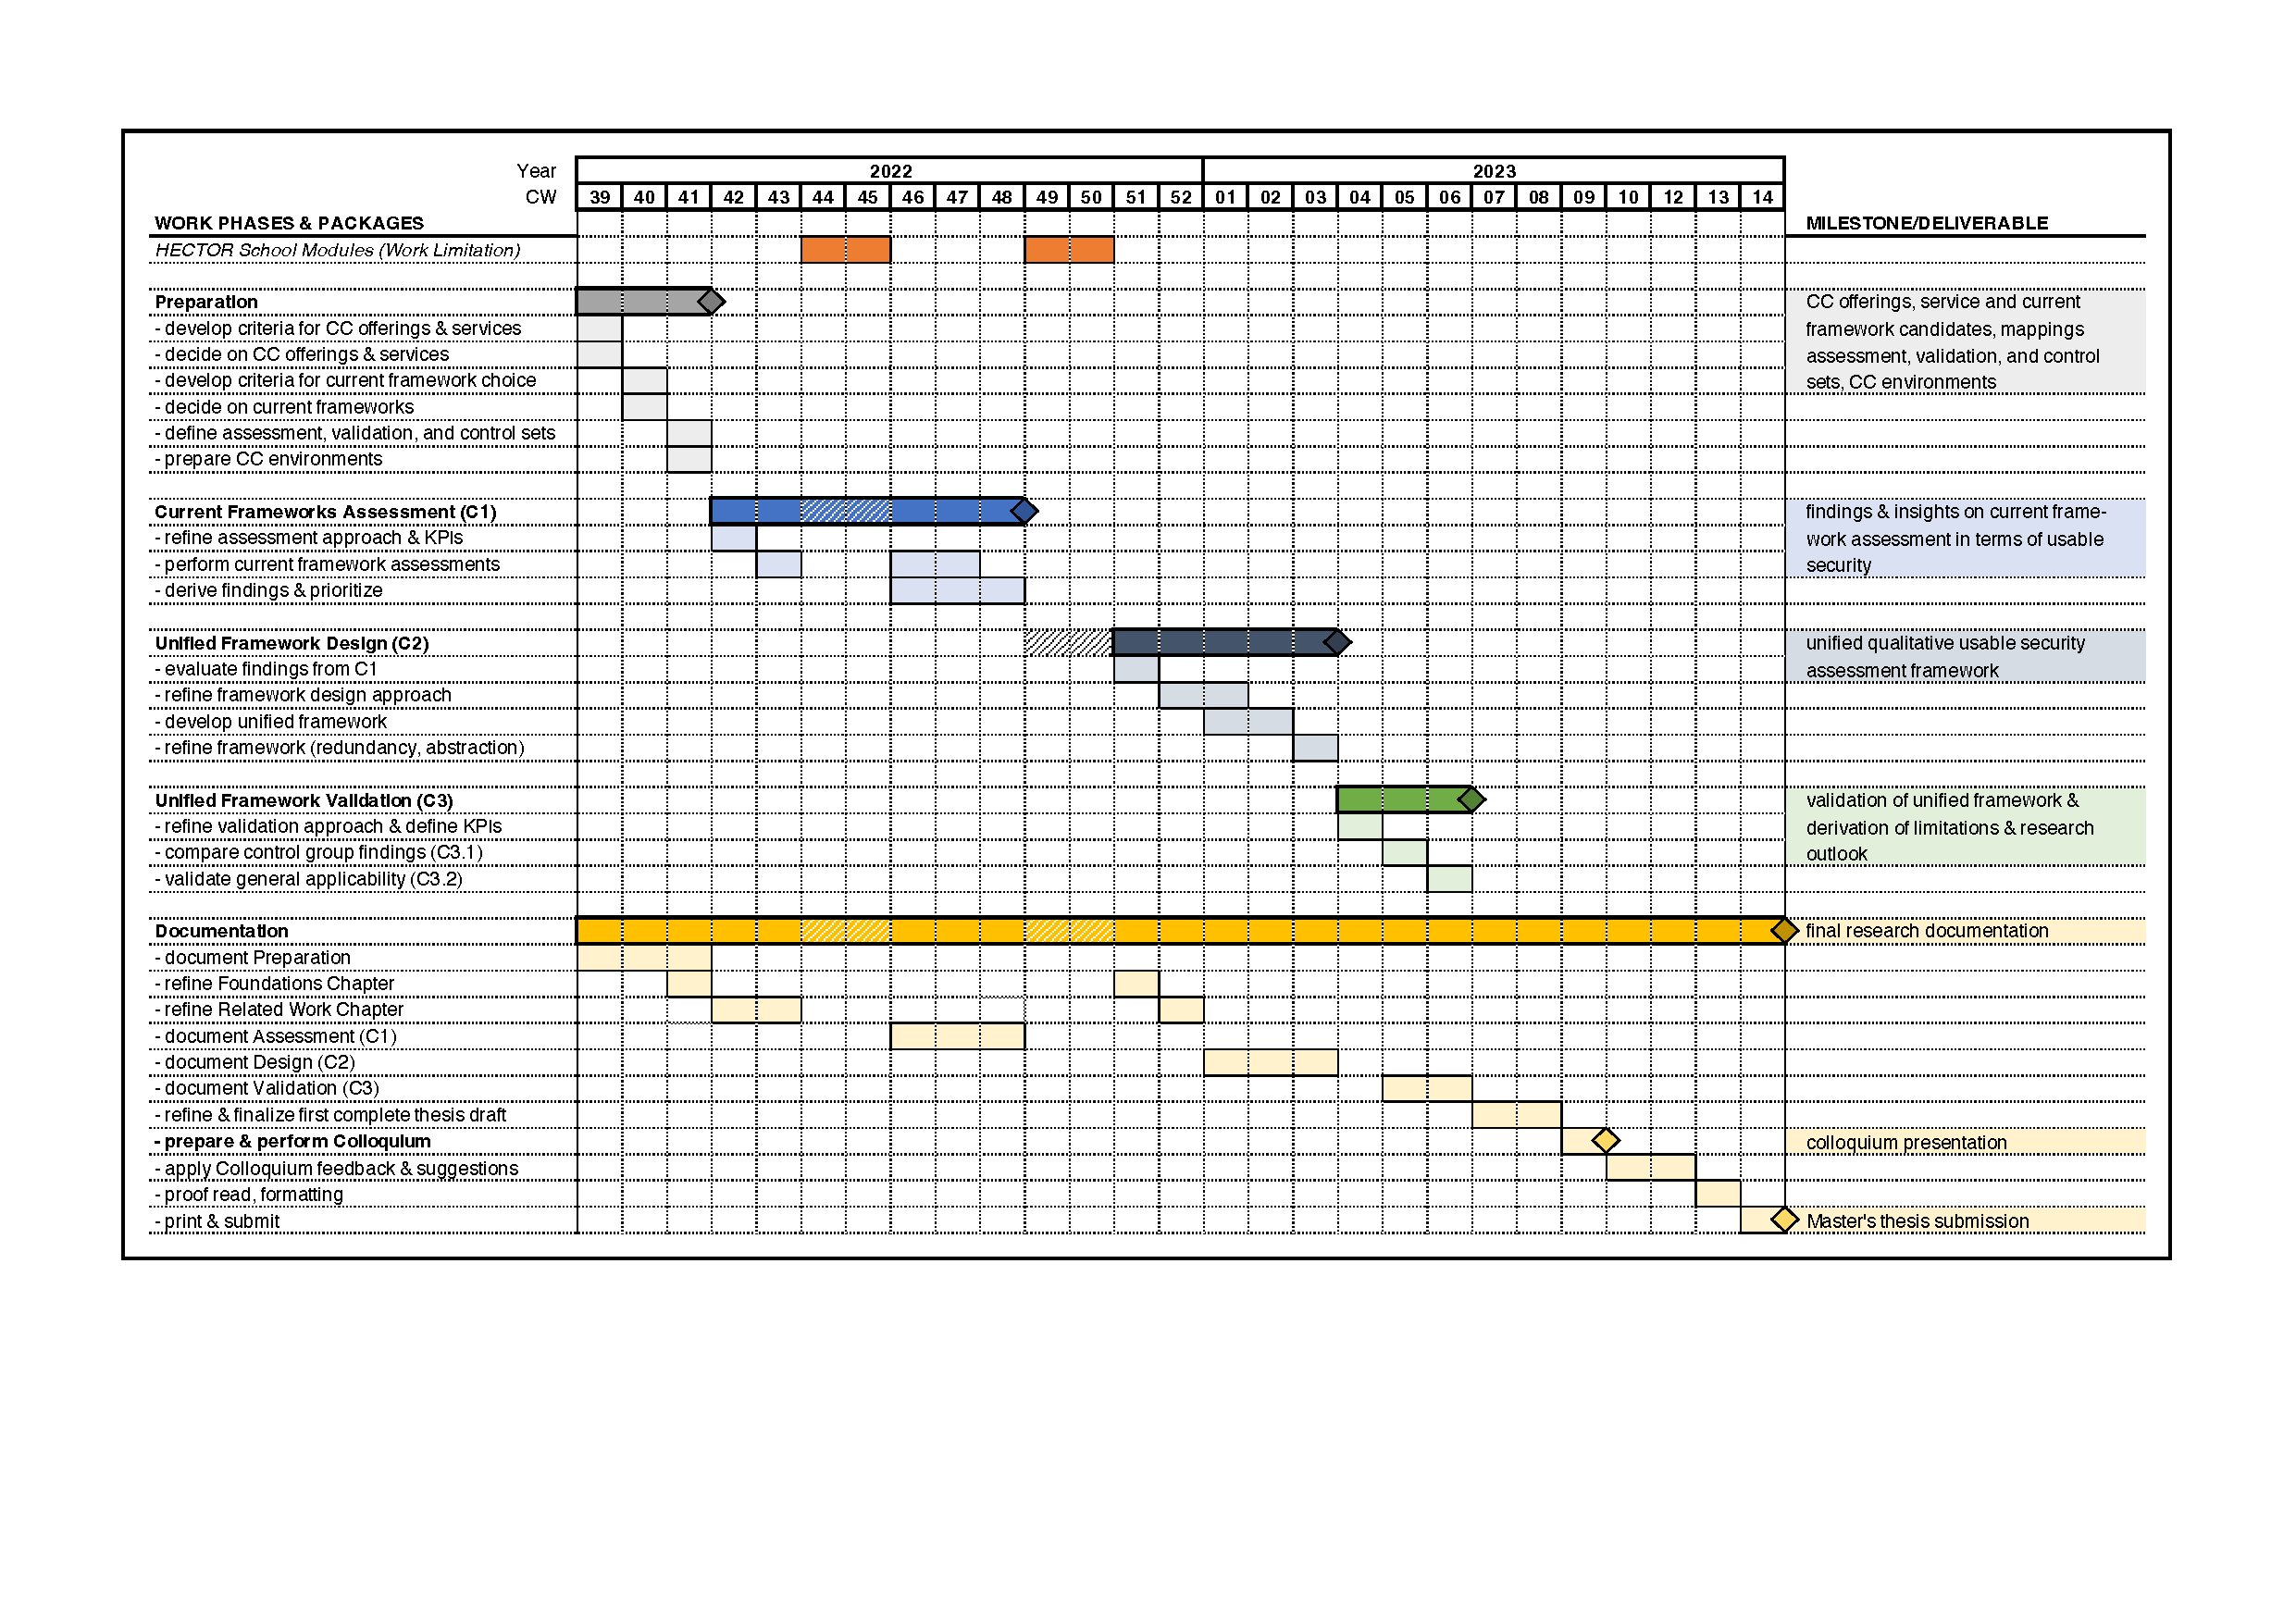
\includegraphics[angle=90,scale=0.5]{content/2-research-proposal/img/gantt.pdf}
		\caption{Preliminary GANTT chart}
		\label{fig:organization-gantt}
	\end{figure}
	\vfill
	\clearpage

	
% = END OF RESEARCH PROPOSAL ===============================================
	